% !TEX encoding = UTF-8
% !TEX TS-program = pdflatex
% !TEX root = ../tesi.tex

%**************************************************************
\chapter{User manual}
\label{cap:user-manual}
%**************************************************************

%**************************************************************
\section{Project setup}

The project will be available at the following GitHub repository: \newline{}
\centerline{\href{https://github.com/RakuJa/Project\_ACCS}{https://github.com/RakuJa/Project\_ACCS}} \newline{}
where a detailed \href{https://github.com/RakuJa/Project_ACCS/blob/main/README.MD}{README} file will explain how to setup the project and the \href{https://github.com/RakuJa/Project_ACCS/releases}{releases} button will list the compiled executables for Ubuntu 18.04.

\section{Login}

The project consists of two distinct programs: one is the server and one is the client.
When booting up the server the user will need to input the port in which you want the server to listen \newline{}
\centerline{ex: ./server 25565} \newline{}

\begin{figure}[!h] 
    \centering 
    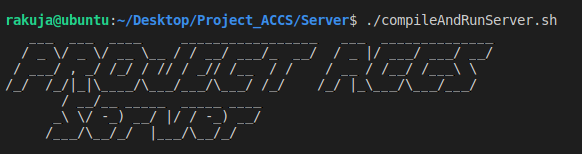
\includegraphics[width=1\columnwidth]{chapter-4/boot_server.PNG} 
    \caption{Prompt when server is booted.}
    \label{fig:booted_server_prompt}
\end{figure}
When booting up the client the user will need to input the address and port in which the server is listening so that the client can connect correctly. \newline{}
\centerline{ex: ./client 127.0.0.1 25565} \newline{}

\begin{figure}[!h] 
    \centering 
    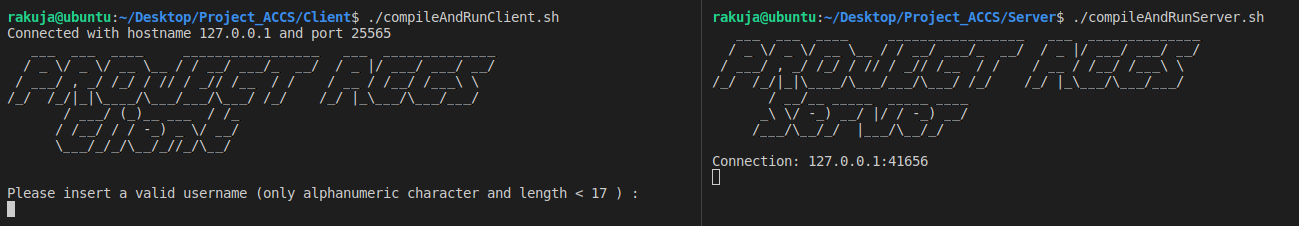
\includegraphics[width=1\columnwidth]{chapter-4/connection_established.PNG} 
    \caption{Connection established correctly.}
    \label{fig:connection_established_prompt}
\end{figure}
\newpage{}
Once the connection is established the user will be prompted with two consecutive inputs:
\begin{enumerate}
	\item \textbf{Username}: the usernames currently registered right now are two: ``Alice'' and ``Daniele'' (Bob was busy);
	\item \textbf{Password}: the password for both the currently registered users is: ``ElPsyKongroo''.
\end{enumerate}

\begin{figure}[!h] 
    \centering 
    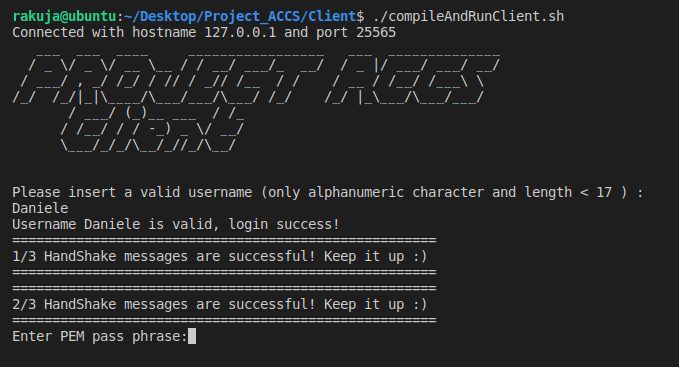
\includegraphics[width=1\columnwidth]{chapter-4/credentials.PNG} 
    \caption{User is prompted to enter credentials.}
    \label{fig:credentials}
\end{figure}

\newpage{}

The client application does not store anything, so credentials will be asked on every boot up. The server is multithreaded and can handle multiple clients.

Once the connection is correctly established the user will be prompted with a success login screen and will be free to carry out all the operation described at \ref{sec:operations}. Each user will have its own remote storage space, indipendent from one another.

\begin{figure}[!h] 
    \centering 
    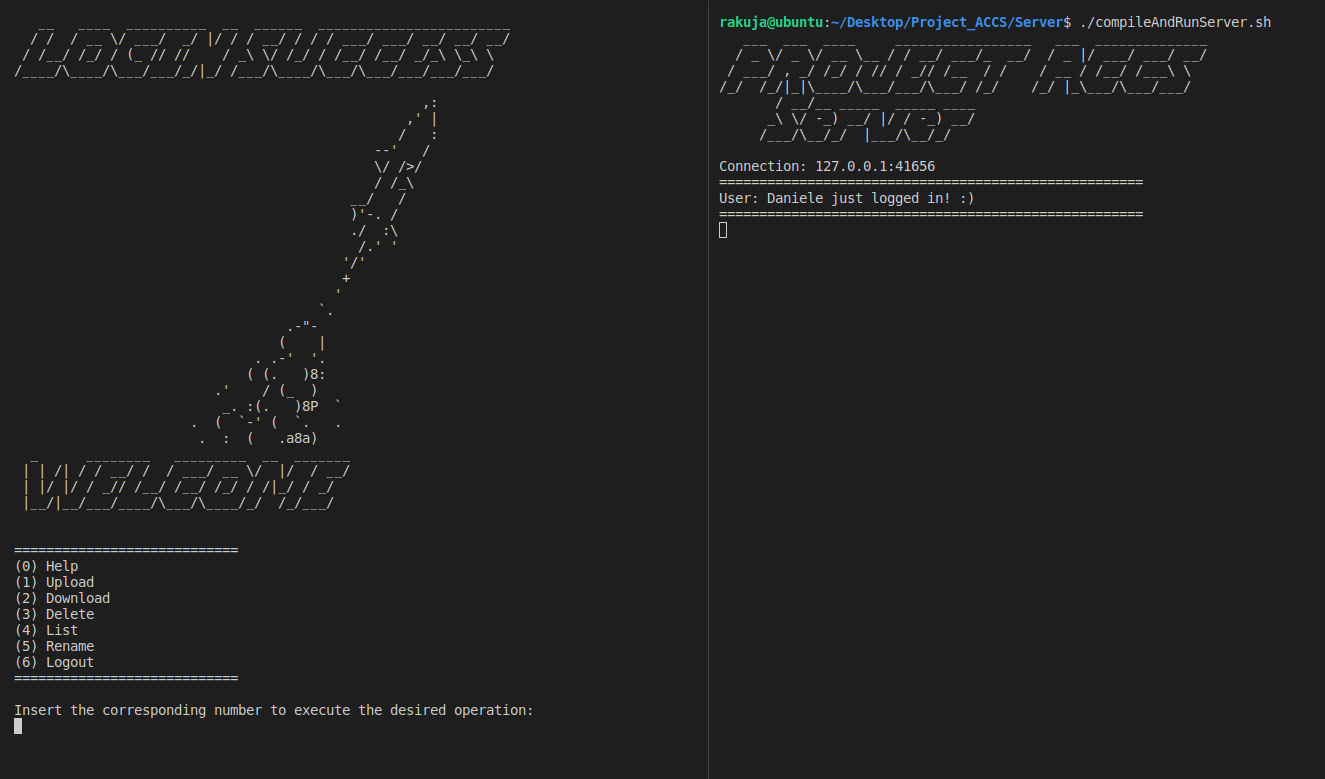
\includegraphics[width=1\columnwidth]{chapter-4/handshake_success.PNG} 
    \caption{Handshake successful message.}
    \label{fig:handshake_success}
\end{figure}
